\documentclass{standalone}

\usepackage{tikz}
\usetikzlibrary{calc}

\begin{document}
  %noformat{
  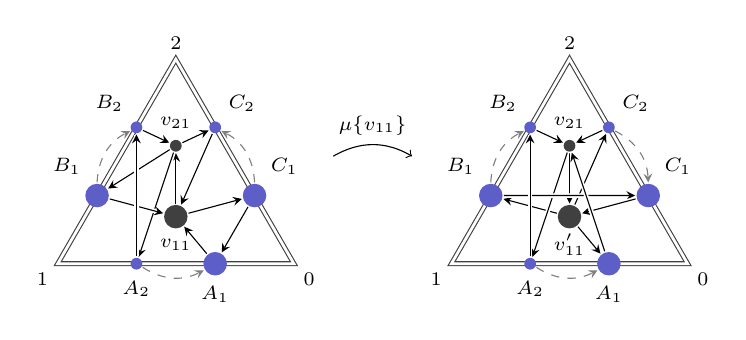
\begin{tikzpicture}
    \tikzstyle{v1} = [circle, outer sep=0.5pt, fill, inner sep=1.5pt]
    \tikzstyle{v2} = [circle, outer sep=0.5pt, fill, inner sep=3.0pt]
    \tikzstyle{unf} = [color=darkgray]
    \tikzstyle{frz} = [color=blue!60!darkgray!70]
    \tikzstyle{r} = [color=red!70!darkgray!70]
    \tikzstyle{e} = [->, >={stealth}, preaction={draw=white, -, ultra thick}]
    \tikzstyle{b} = [fill, fill opacity=0.0, circle, outer sep=0.5pt, inner sep=1.5pt]
    \tikzstyle{te} = [color=darkgray, double distance=1pt]
    \tikzstyle{h} = [dashed, color=gray, ->, >={stealth}]

    \tikzset{font=\scriptsize}

    \begin{scope}[shift={(0,0)}]
      \coordinate[label={330:$0$}] (l_0) at (-30:1.7321);
      \coordinate[label={210:$1$}] (l_1) at (210:1.7321);
      \coordinate[label={ 90:$2$}] (l_2) at ( 90:1.7321);

      \draw[te] (l_0) -- (l_1) -- (l_2) -- cycle;

      \node[v2, frz, label={120:$B_1$}   ] (B1)  at ($ (l_1) + ( 60:1.0)$) {};
      \node[v1, frz, label={120:$B_2$}   ] (B2)  at ($ (l_1) + ( 60:2.0)$) {};
      \node[v1, frz, label={270:$A_2$}   ] (A2)  at ($ (l_1) + (  0:1.0)$) {};
      \node[v2, frz, label={270:$A_1$}   ] (A1)  at ($ (l_1) + (  0:2.0)$) {};
      \node[v2, frz, label={ 60:$C_1$}   ] (C1)  at ($ (l_2) + (-60:2.0)$) {};
      \node[v1, frz, label={ 60:$C_2$}   ] (C2)  at ($ (l_2) + (-60:1.0)$) {};
      \node[v2, unf, label={270:$v_{11}$}] (v11) at ($ (l_2) + (270:2.0)$) {};
      \node[v1, unf, label={ 90:$v_{21}$}] (v21) at ($ (l_2) + (270:1.1)$) {};

      \draw[h] (A2) to[bend right] (A1);
      \draw[h] (B1) to[bend left] (B2);
      \draw[h] (C1) to[bend right] (C2);

      \draw[e] (v11) -- (v21);
      \draw[e] (v11) -- ( C1);
      \draw[e] (v21) -- ( B1);
      \draw[e] (v21) -- ( C2);
      \draw[e] (v21) -- ( A2);
      \draw[e] ( B1) -- (v11);
      \draw[e] ( B2) -- (v21);
      \draw[e] ( C1) -- ( A1);
      \draw[e] ( C2) -- (v11);
      \draw[e] ( A1) -- (v11);
      \draw[e] ( A2) -- ( B2);
    \end{scope}

    \draw[->] (2,0.5) to[bend left=30] node[midway, above] {$\mu\{v_{11}\}$} (3,0.5);

    \begin{scope}[shift={(5,0)}]
      \coordinate[label={330:$0$}] (l_0) at (-30:1.7321);
      \coordinate[label={210:$1$}] (l_1) at (210:1.7321);
      \coordinate[label={ 90:$2$}] (l_2) at ( 90:1.7321);

      \draw[te] (l_0) -- (l_1) -- (l_2) -- cycle;

      \node[v2, frz, label={120:$B_1$}   ] (B1)  at ($ (l_1) + ( 60:1.0)$) {};
      \node[v1, frz, label={120:$B_2$}   ] (B2)  at ($ (l_1) + ( 60:2.0)$) {};
      \node[v1, frz, label={270:$A_2$}   ] (A2)  at ($ (l_1) + (  0:1.0)$) {};
      \node[v2, frz, label={270:$A_1$}   ] (A1)  at ($ (l_1) + (  0:2.0)$) {};
      \node[v2, frz, label={ 60:$C_1$}   ] (C1)  at ($ (l_2) + (-60:2.0)$) {};
      \node[v1, frz, label={ 60:$C_2$}   ] (C2)  at ($ (l_2) + (-60:1.0)$) {};
      \node[v2, unf, label={[label distance=-2pt]270:$v_{11}'$}] (v11) at ($ (l_2) + (270:2.0)$) {};
      \node[v1, unf, label={ 90:$v_{21}$}] (v21) at ($ (l_2) + (270:1.1)$) {};

      \draw[h] (A2) to[bend right] (A1);
      \draw[h] (B1) to[bend left] (B2);
      \draw[h] (C2) to[bend left] (C1);

      \draw[e] (B2)  -- (v21);
      \draw[e] (v11) -- (B1);
      \draw[e] (v11) -- (C2);
      \draw[e] (v11) -- (A1);
      \draw[e] (v21) -- (v11);
      \draw[e] (v21) -- (A2);
      \draw[e] (B1)  -- (C1);
      \draw[e] (B2)  -- (v21);
      \draw[e] (C1)  -- (v11);
      \draw[e] (C2)  -- (v21);
      \draw[e] (A1)  -- (v21);
      \draw[e] (A2)  -- (B2);
    \end{scope}
  \end{tikzpicture}
  %}noformat
\end{document}
